\chapter{2D Triangulation Data Structure} 
\label{user_chapter_2D_Triangulation_Data_Structure}
\label{Chapter_2D_Triangulation_Data_structure}
\minitoc



\section{Definition}
\label{2D_TDS_Definition}
A triangulation data structure is a data structure designed
to handle the representation of a two dimensional
triangulation. The concept of triangulation data structure
was primarily designed to serve as a data structure
for \cgal\ 2D triangulation classes which are triangulations
embedded in a plane.
However it appears that the concept is more general
and can be used for any  orientable triangulated surface
without boundary, whatever may be the dimensionality
of the space the trianguation is embedded in.


\subsection{A data structure based on faces and vertices}

The representation of \cgal\ 2D triangulations is based on faces and vertices,
Edges are only implicitely 
represented trough the adjacency relations betwen two
faces.

The triangulation data structure can be seen 
as a container for faces and vertices
maintaining incidence and adjacency relations
among them.

Each triangular face gives access to its three incident vertices 
and to its three adjacent faces. 
Each vertex gives access to one of its incident faces
and through that face to the circular list of its incident faces.

The three vertices of a face are indexed with 0, 1 and 2.
The neighbor of a face are also 
indexed with 0,1,2 in such a way that the neighbor indexed by \ccc{i}
is opposite to the vertex with the same index.

Each edge has two implicit representations : the edge
of a face \ccc{f}  which is opposed to the vertex indexed \ccc{i},
can be represented as well as an edge of the \ccc{neighbor(i)} of 
\ccc{f}. See Figure~\ref{2D_Triangulation_Fig_neighbors1}.

 \begin{figure}
\begin{ccTexOnly}
    \begin{center}
     \includegraphics[width=6cm]{rep_bis.eps} 
    \end{center}
\end{ccTexOnly} 
    \caption{Vertices and neighbors. The function \ccc{ccw(i)}
and \ccc{cw(i)} compute respectively $i+1$ and $i-1$ modulo 3.
    \label{2D_TDS_Fig_neighbors1}}
  \begin{ccHtmlOnly}
<CENTER>
<img border=0  src=rep_bis.gif width=400 align=center alt="Neighbors">
</CENTER>
\end{ccHtmlOnly} 
\end{figure}



This kind or representation of simplicial complexes extends in any
dimension. More precisely, in dimension $d$, the data structure
will explicitely represents cells (i. e. faces of maximal dimension) 
and vertices (i. e. faces of dimension 0).
All faces of dimension between $1$ and $d-1$
will have an implicit representation.
The 2D triangulation data structure can represent simplicial complexes
of dimension 2, 1 or 0.

\subsection{The set of faces and vertices}
 The set of faces  maintained by a 2D triangulation 
data structure is such that each edge
is incident to two faces. In other words,
the set of maintained faces 
is topologically
equivalent to a two-dimensional triangulated sphere.

This rules extends to  lower dimensional triangulation data structure
arising in degenerate cases or when the triangulations
have less than three vertices.
A one dimensional triangulation structure maintains a set of vertices
 and edges which forms a ring 
topologically equivalent to a $1$-sphere.

A zero dimensional triangulation data structure
only includes two adjacent vertices 
that is
topologically equivalent to a $0$-sphere.


\section{The Concept of Triangulation Data Structure}
\label{2D_TDS_Concept}
A model of \ccc{TriangulationDataStructure_2}
can be seen has a container for the 
faces and vertices of the triangulation.
This class is also responsible for the combinatorial
integrity of the triangulation. This means that
the triangulation data structure 
maintains  proper incidence and adjacency relations among the vertices
and faces of a triangulation while
combinatorial modifications
of the triangulation are performed.
The term  combinatorial modification 
refers to  operations which do not 
involve any knowledge about the geometric embedding of the triangulation.
For example, the  
insertion of a new vertex in a given face, or in a given edge,
the suppression
of a vertex of degree three,  the flip of two edge are 
examples of combinatorial operation performed at the data structure level.


The triangulation data structure 
is required to provide :
\begin{itemize}
\item
the types \ccc{Vertex} and \ccc{Face} for the the vertices
and faces of the triangulations
\item the type \ccc{Vertex_handle} and \ccc{Face_handle}
through which the vertices and faces of the triangulation are accessed.
\item
iterators to visit all the vertices, edges and faces
of the triangulation,
\item
circulators to visit all the vertices, edges and faces
incident to a given vertex
\end{itemize}


The triangulation data structure is responsible 
for the creation and removal of faces and vertices 
(memory management).
It provides function that gives the number of faces, edges and
vertices
of the triangulation.

The triangulation data structure provides member functions
to perform the following  combinatorial transformation of the triangulation:\\
-- flip of two adjacent faces, \\
-- addition  of a new vertex splitting a given face 
see Figure~\ref{2D_TDS_Fig_insertion},\\
--  addition  of a new vertex splitting a given edge,\\
-- addition of a new vertex raising by one the dimension of a degenerate
-- lower dimensional triangulation, \\
-- removal of a vertex incident to three faces, \\
-- removal of a vertex lowering the dimension of the triangulation.\\


%\begin{figure}
%\begin{ccTexOnly}
%\begin{center} %\IpeScale{70} \Ipe{Flip.ipe} \end{center}
%\input{flip.ltex}
%\end{center}
%\end{ccTexOnly} 
%\caption{Flip. \label{{2D_Triangulation_fig_flip_bis}}

%\begin{ccHtmlOnly}
%<CENTER>
%<img border=0 src=Flip.gif align=center alt="Flip">
%</CENTER>
%\end{ccHtmlOnly} 
%\end{figure}



\begin{figure}
\begin{ccTexOnly}
%\begin{center} \IpeScale{70} \Ipe{Three.ipe} \end{center}
\begin{center} \documentclass{article}
\documentclass{article}
\documentclass{article}
\input{tmp.inputs}
\pagestyle{empty}
\begin{document}
\input{tmp.pstex_t}
\end{document}

\pagestyle{empty}
\begin{document}
\documentclass{article}
\input{tmp.inputs}
\pagestyle{empty}
\begin{document}
\input{tmp.pstex_t}
\end{document}

\end{document}

\pagestyle{empty}
\begin{document}
  \begin{tabular}{ccc}
    \input{insert1.pstex_t} &
    \input{insert2.pstex_t} &
    \input{insert3.pstex_t}\\
  {\small (a)} & {\small (b)} & {\small (c)}\\
  \end{tabular}
\end{document}
 \end{center}
\end{ccTexOnly} 
\caption{Insertion of a new vertex, splitting a face}
 \label{2D_TDS_Fig_insertion}
\begin{ccHtmlOnly}
<CENTER>
<img border=0 src=Three.gif align=center alt="Insertion">
</CENTER>
\end{ccHtmlOnly} 
\end{figure}


\section{The Default Triangulation Data Structure}
\label{2D_TDS_default}

\cgal\ provides the class
\ccc{CGAL::Triangulation_data_structure_2<Vb,Fb>}
as a default triangulation data structure.


\subsection{Flexibility}
In oder to provide flexibility, the default triangulation data
structure is templated by two parameters 
which stands respectively for a vertex base class and a face base
class.
The concept 
\ccc{TriangulationDSVertexBase_2} and 
\ccc{TriangulationDSFaceBase_2} describe the requirements for the
base vertex and face classes of a triangulation data structure.

The triangulation data structure 
derives from thoses base classes the
vertex and face classes from thoses base classes.
This design  allows the user to plug in the
triangulation data structure
his own base classes tuned for  his application.

\subsection{The cyclic dependancy of template parameters}
 Since adjacency and incidence relation are stored in vertices and
faces,
the vertex and face base classes have to know the types
of handles on faces and vertices provided by the triangulation data
structure.
Therefore , vertex and base classes need to be templated 
by the triangulation data structure. Because the triangulation
data structure 
is itself templated by the vertex and base classes this induces
a cyclic dependancy.
See figure~\ref{2D_TDS_Fig_three_levels_2}.

\begin{figure}
\begin{ccTexOnly}
\begin{center}
\includegraphics[width=13cm]{threelevels2.eps}
\end{center}
\end{ccTexOnly}
\caption{The cyclic dependency in triangulations software design.
\label{2D_TDS_Fig_three_levels_2}}
\begin{ccHtmlOnly}
<CENTER>
<br>
<img border=0 src=threelevels2.gif align=center alt="Three_levels">
</CENTER>
\end{ccHtmlOnly}
\end{figure}


\subsection{The rebind mecanism}

The solution proposed by \cgal\ to resolve this cyclic dependency
is based on a rebind mecanism similar to the mecanism used in the 
standard allocator class std::allocator.
The vertex and face base classes plugged in the instantiation of a
triangulation data structure are themselves instantiated with a
fake data structure. The triangulation data structure
will then rebind  these classes, plugging itself
at the place of the fake data structure, before using them
to derive  the vertex and face classes. The rebinding is performed
through a nested template class  \ccc{Rebind_TDS} in the vertex and
face base class, which provide the rebound class
as a type called  \ccc{Other}.

Here is how it works schematically. First, here is the rebinding
taking place in the triangulation data stucture.
\begin{ccExampleCode}
template < class Vb, class Fb >
class Triangulation_data_structure
{
  typedef Triangulation_data_structure<Vb,Fb>    Self;

  // Rebind the vertex and cell base to the actual TDS (Self).
  typedef typename Vb::template Rebind_TDS<Self>::Other  VertexBase;
  typedef typename Fb::template Rebind_TDS<Self>::Other  FaceBase;

  // ... further internal machinery leads to the final public types:
public:
  typedef ...  Vertex;
  typedef ...  Face;
  typedef ...  Vertex_handle;
  typedef ...  Face_handle;
};
\end{ccExampleCode}

Then, here is the vertex base class with its nested 
 \ccc{Rebind_TDS} template class and its template parameter
set by default to an an internal type faking a  triangulation data 
structure.
\begin{ccExampleCode}
template < class TDS = an internal type faking a triangulation data 
structure >
class Vertex_base
{
public:
  template < class TDS2 >
  struct Rebind_TDS {
    typedef Vertex_base<TDS2>    Other;
  };
...
};
\end{ccExampleCode}
Imagine an analog \ccc{Face_base} class.
The triangulation data structure is then instantiate as follows~:
\begin{ccExampleCode}
typedef Triangulation_data_structure< Vertex_base<>, Face_base<> > TDS;
\end{ccExampleCode}


\subsection{Making use of the flexibility}

There is several possibilities to make use
of the flexibility offered by 
the triangulation data structure.
\begin{itemize}
\item{} First, when the user needs to have,
in vertices and faces, additionnal informations 
which do not depend on types defined by the
triangulated data structure,  predefined classes 
\ccc{Triangulation_vertex_base_with_info}
and \ccc{Triangulation_face_base_with_info} can be plugged in.
Those classes have a template parameter \ccc{Info} to be instantiated
by a user defined type. They
store a data member of this type and gives acces to it.
\item{} Second, the user  can derive 
his own base classes from the default base
classes :
\ccc{Triangulation_ds_vertex_base_2}, and
\ccc{Triangulation_ds_cell_base_2}
are the default base classes to be plugged in a triangulation 
data structure used alone.
Triangulation classes requires a data strucure in which
other base classes have been plugged it. The default base classes
for most of the triangulation classes are
\ccc{Triangulation_vertex_base_2}, and \ccc{Triangulation_face_base_2}
are the default base classes to be used when the triangulation data
structure is plugged in a triangulation class.

When derivation is used, the rebind mecanism is slightly
more involved, because it is necessary to rebind the  base class
itself. However the user will be able to use in his classes
references to types provided by the triangulation data structure.
For example,
\begin{ccExampleCode}
template < class Gt, class Vb = CGAL::Triangulation_vertex_base_2<Gt> >
class My_vertex_base 
  : public  Vb
{
public :
  template < typename TDS2 >
  struct Rebind_TDS {
    typedef typename Vb::template Rebind_TDS<TDS2>::Other    Vb2;
    typedef My_vertex_base<Gt,Vb2>                           Other;
  };

  typedef typename Vb::Triangulation_data_structure    Tds;
  typedef typename Tds::Vertex_handle                  Vertex_handle;
  ......
};
\end{ccExampleCode}

\item{} At last the user can write his own base classes.
If the triangulation data structure is used alone, 
the requirements for the base classes are described by the concepts
\ccc{TriangulationDSVertexBase_2} 
and \ccc{TriangulationDSFaceBase_2}\lcTex{, 
 documented \ccRefPage{TriangulationDSVertexBase_2} and
\ccRefPage{TriangulationDSFaceBase_2}}.
If the triangulation data structure is plugged into a triangulation
class,
the concepts for the vertex and base classes depends on the
triangulation class. The most basic concepts, valid for
basic and Delaunay triangulations are \ccc{TriangulationVertexBase_2} 
and \ccc{TriangulationFaceBase_2}\lcTex{, documented 
\ccRefPage{TriangulationVertexBase_2}
and \ccRefPage{TriangulationFaceBase_2}}.
\end{itemize}

 See section~\ref{Section_2D_Triangulations_Flexibility} 
for examples of using the triangulation data structure flexibility.



